\documentclass[12pt]{beamer}

\usepackage[orientation=portrait, size=a0, scale=1.25]{beamerposter}

\usepackage[spanish]{babel}
\usepackage{amsmath, amsfonts, amssymb, bm}
\usepackage{graphicx}
\usepackage{xcolor}
\usepackage{setspace}
\usepackage{lipsum, blindtext}
\usepackage{ragged2e}
\usepackage{upgreek}
\usepackage[many]{tcolorbox}

\usetheme{Madrid}
\usecolortheme{seahorse}

%\geometry{left=2cm, right=2cm, top = 0cm, bottom =0cm}

\definecolor{azul}{rgb}{0.17,0.40,0.69}
\definecolor{verde}{RGB}{000,096,006}
\definecolor{gris}{rgb}{0.18, 0.31, 0.31}
\definecolor{rojo}{RGB}{194,000,009}
\definecolor{azul1}{RGB}{004,122,165}
\definecolor{cel}{RGB}{204,221,236}
\definecolor{mor}{RGB}{144,144,243}
\definecolor{azl}{RGB}{000,151,196}
\definecolor{azc}{RGB}{006,109,150}
\definecolor{azr}{RGB}{013,055,090}


%\beamertemplateshadingbackground{white}{mor!60}
%\usebackgroundtemplate{
%
\includegraphics[width=1.0\paperwidth, height=1.0\paperheight]{figures/background.jpg}
%}

%\setbeamercolor{block title}{bg=azul1, fg=white}
%\setbeamercolor{block body}{bg = cel, fg=black}

%\setbeamercolor{block body example}{bg= verde!10, fg=black}
%\setbeamercolor{block title example}{bg = verde!80, fg=white}

%\setbeamercolor{block title alerted}{bg=rojo!80, fg=white}
%\setbeamercolor{block body alerted}{bg =rojo!10 , fg=black}

%\setlength{\columnsep}{30pt}


\title{Un poster construido en \LaTeX usando beamer}
\author{González-Aguirre, J.C.\inst{1}, Díaz M.A\inst{2}.}
\institute[TECNM, RC]{
	\inst{1} Universidad Juárez Autónoma de Tabasco. \\
	\inst{2} \'{E}cole Supérieure de M\'{e}canique et d’A\'erotechnique Institute Pprime.
}

\begin{document}

	\begin{frame}[t]
	
		\begin{table}[t]
			\centering
			\begin{tabular}{ccc}
				\begin{minipage}{0.25\linewidth}
					\begin{figure}[h]
						\centering
						
\includegraphics[scale=0.75]{figures/TecNM.png}
					\end{figure}
				\end{minipage}
			&
			\begin{minipage}{0.5\linewidth}
				\begin{center}
					{\Huge  {\color{blue} \textbf{\inserttitle}}}\\ \vspace{1cm}
					{\huge  \insertauthor}\\ \vspace{0.5cm}
					{\large \textit{\insertinstitute}}
				\end{center}
			\end{minipage}
			&
			\begin{minipage}{0.25\linewidth}
				\begin{figure}[h]
					\centering
					
\includegraphics[scale=1.1]{figures/carbonifera.png}
				\end{figure}
			\end{minipage}
			
			\end{tabular}
		\end{table}
	
	\begin{block}{{\sc{\Large Introducción}}}
		%\justifiying
		  The study of sediment transport  focusses on understanding the relationship that exists between the 	movement of water and the movement of sedimentary materials. In this work, this study is carried out by analysing  a system of balance laws consisting in the mass and momentum conservation equations for the water-sediment mixture, the mass conservation equation 
for sediment in suspension and the Exner equation for the morphological evolution. In order to take into account the bed-load transport, the Meyer-Peter \& M\"uller formulation is employed.
We solve numerically the system using the path conservative framework  which can be adapted to accurately capture shocks and sharp fronts.
	\end{block}
	
	\begin{columns}[t]
		% Primera columna
		\begin{column}{0.32\linewidth}
			
			%% 
			\begin{block}{{\Large Mathematical model}}
				
				\begin{center}
				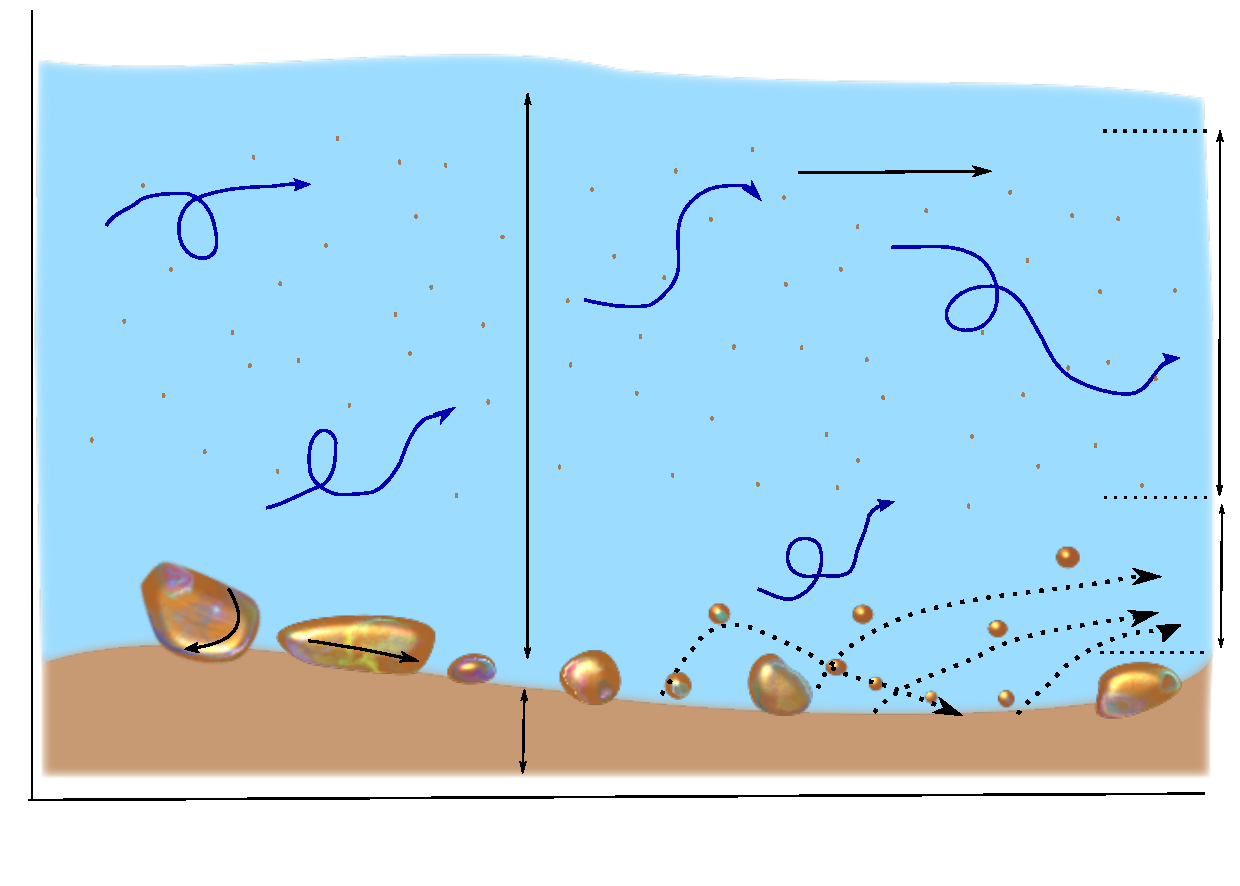
\includegraphics[width=1.0\textwidth]{figures/monito.pdf}
					\put(-490,330){$h(x,t)$}
					\put(-490,80){$b(x,t)$}
					\put(-250,420){$u(x,t)$}
					\put(-550,160){Sliding}
					\put(-650,192){Rolling}
					\put(-220,170){Jumping}
					\put(-680,500){$\eta(x,t) = h(x,t)+b(x,t)$, free surface of water.}
				\end{center}
				\vspace{-1.5cm}
				
				\begin{alertblock}{{\bf Mathematical model}}
					\begin{equation}\label{2d1}
						\partial _t h + \partial _x (hu) + \partial _y (hv) = \frac{\phi _b }{1-p},
					\end{equation}	
					
					\begin{equation}\label{2d2}
						\partial  _t (h\rho)+ \partial _x (h\rho u) + \partial _y (h\rho v) = \frac{\phi _b}{1-p}\rho_b,
					\end{equation}
				\begin{equation}\label{2d3}
					\begin{split}
					 \partial_t (h\rho u) + \partial_x\left( h\rho u^2 + \frac{1}{2}gh^2\rho \right) + \partial _y (h\rho uv)\\ = - gh\rho \partial_x b + \uptau _u
					+\rho \phi_b\frac{u}{2},
				\end{split}
			\end{equation}	
			
			\begin{equation}\label{2d4}
				\begin{aligned}
				& \ \partial _t (h\rho v) + \partial _x (h\rho uv) + \partial_y \left( h\rho v^2 +  \frac{1}{2}gh^2\rho \right) &\\& = - gh\rho \partial_y b + \uptau _v 
				+\rho \phi_b\frac{v}{2},
				\end{aligned}
			\end{equation}
			\begin{equation}\label{2d5}
				\partial_t b + \frac{1}{1-p}\left( \partial _x q_b + \partial _y q_b \right) = -\frac{\phi_b}{1-p},
			\end{equation}		
				\end{alertblock}
				\vspace{0.5cm}
				\begin{exampleblock}{{\it where}}
				 where, $h$ is the depth of water, $\mathbf{u}=(u,v)$ is the  flow velocity, $\rho$ is the density of water sediment mixture, 
$b(x,t)$ is the bottom thickness, $g$ is the gravitational aceleration,
$p$ is the porosity of sediment bottom, $\phi _b$ is the sediment flux between the bottom and the fluid,
$\rho _b$ is the density of saturated bottom, $\uptau _u$ and $\uptau _v$ are bottom frictions effects on $x$ and $y$ directions, 
respectively and $(q_{b,x},q_{b,y})$ is the bed load discharge.

				\end{exampleblock}
				\vspace{0.5cm}
			\end{block}
		\end{column}
		
		% Segunda columna
		\begin{column}{0.32\linewidth}
			
			%% 
			\begin{block}{{\Large Mathematical model}}
			
			\end{block}
		\end{column}
		
		% Tercera columna
		\begin{column}{0.32\linewidth}
			
			%% 
			\begin{block}{{\Large Mathematical model}}
			
			\end{block}
		\end{column}
	\end{columns}	
	
	
	\end{frame}



\end{document}